\documentclass[a4paper, 15pt]{article}
\usepackage[left=0.85in, right=0.85in, top=0.5in, bottom=0.95in]{geometry}
\usepackage[T1]{fontenc}
\usepackage[utf8]{inputenc}
\usepackage[italian]{babel}
\usepackage[none]{hyphenat} % no sillabazione 
\usepackage{multicol} %testo su più colonne
\usepackage{enumerate}
\usepackage{enumitem}
\usepackage{mdwlist} %suspend enumerate \suspend{} \resume{}
\usepackage{lipsum} %testo random per verifica \lipsum
\usepackage{graphicx, nicefrac}
\usepackage{wrapfig2}
\usepackage{amsmath}
\usepackage{mathtools}
\usepackage{amssymb}
\usepackage{amsthm} %teoremi e dimostrazioni e definizioni
\usepackage{cases}
\usepackage{gensymb} %simboli come ° = \degree  etc etc
\usepackage{cancel} %permette di fare semplificazioni utilizzando il comando \cancel{expression}
\usepackage{subcaption}
\usepackage{hyperref}
\hypersetup{
	colorlinks=true,
	linkcolor=blue,    
	urlcolor=blue,
	%pdfpagemode=FullScreen, %il pdf generato non si avvia a schermo intero
}
\urlstyle{same}
\usepackage{changepage}
\usepackage{lastpage, epstopdf}
\usepackage{fancyhdr}
\usepackage{tcolorbox}
%\usepackage{background} %non utilizza lo sfondo con "draft"
\usepackage{color} % testo colorato \textcolor{'ColorCode'}{'testo'}
\usepackage{setspace} % in questo modo posso settare lo spoazio dell'indice \begin{spacing}{0.95}	
\usepackage{changepage}
\usepackage{lastpage, epstopdf}
\usepackage{fancyhdr}
\usepackage{tcolorbox}
%\usepackage{background}
%%%%%%%%%%%%%%%%%%%%%%%%%%%%%%%%%%%%%%%%%%%% AMBIENTE TIKZ 
\usepackage{tikz} %disegni e mappe
\usetikzlibrary{patterns}
\usepackage{pgfplots}
\pgfplotsset{compat=1.15}
\usepackage{mathrsfs}
\usetikzlibrary{arrows,decorations.markings,arrows.meta, decorations.text}
\usepackage{circuitikz}
\tikzset{immagine/.style={%
		above right, inner sep=0pt, outer sep=0pt},
	testo/.style={fill=white, align=center,
		fill opacity=0.6, text opacity=1, below,
		font=\sffamily\bfseries\footnotesize}}
\raggedbottom
\setlength{\parindent}{0pt}
%%%%%%%%%%%%%%%%%%%%%%%%%%%%%%%%%%%%%%%%%%%% SIUNITX 
\usepackage{siunitx}
%========TEOREMI========%
\newtheorem*{thm}{Teorema}
\newtheorem*{en}{Enunciato}
\newtheorem*{definizione}{Definizione}
\newtheorem*{cor}{Corollario}
%========OPERATORI&COMANDI========%
\DeclareMathOperator{\rk}{rk}
\DeclareMathOperator{\im}{Im}
\DeclareUnicodeCharacter{20AC}{\EUR}
\newcommand{\cmark}{\ding{51}}
\newcommand{\xmark}{\ding{55}}
\newcommand{\compresslist}{ % Define a command to reduce spacing within itemize/enumerate environments, this is used right after \begin{itemize} or \begin{enumerate}
				\setlength{\itemsep}{1pt}
				\setlength{\parskip}{0pt}
				\setlength{\parsep}{0pt}
			}
\newcommand{\ra}[1]{\renewcommand{\arraystretch}{#1}} %stretcho le tabelle
			
%\renewcommand{\arraystretch}{2.5} % Da copiaincollare prima di ambienti array per ampliarli un po'
%\setlength{\jot}{10pt} % affecting the line spacing in the environment SPLIT
			
\begin{document}
\setcounterpageref{secnumdepth}{0}	% NON NUMERO I CAPITOLI
\setcounter{tocdepth}{5} % INCLUDO addirittura I sotto-PARAGRAFI
\tableofcontents 
\newpage

\part{6.MISURE DI CORRENTE, TENSIONE e RESISTENZA}
\section{Misure di corrente}
\subsection{Galvanometro}	
\begin{adjustwidth}{2in}{}
		Il galvanometro è il dispositivo elettromeccanico alla base degli strumenti per
		la misura della corrente (amperometri) e della tensione (voltmetri). 
		\[i\rightarrow \boxed{\text{Galvanometro}}\rightarrow\theta \]
		Tale strumento riceve in input una corrente che trasforma, attraverso lo schema di seguito, in una variazione angolare su di un display. 		
		\begin{figure}[H]
			\centering
			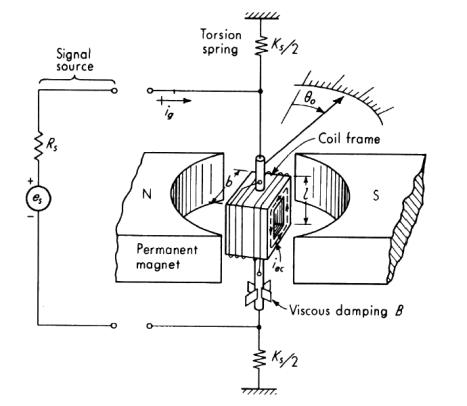
\includegraphics[width=0.5\linewidth]{fig/screenshot001}

			\label{fig:screenshot001}
		\end{figure}
		Un nucleo ferromagnetico avvolto di spire è posto tra un campo magnetico, il nucleo ruoterà a causa della corrente che percorrendo le spire genererà un momento magnetico mentre due molle torsionali che fissano il nucleo al telaio manterranno il nucleo in sede. Un indicatore solidale al nucleo indicherà l'angolo di rotazione. \newline 
		
		L'equazione che governa il moto è:
		\[F = i\vec{l}\times \vec{B}\]
		Più spire in un campo magnetico uniforme imposto generano un momento di rotazione dato da:
		\[ M = n\cdot ilbB\]
		Bene notare che l'unica grandezza qui a variare è la corrente, oggetto di misura, il campo magnetico è imposto e noto. \newline 
		
		Da cosa sarà impedita la rotazione della spira? Dalle molle torsionali solidali al telaio che applicheranno un momento pari a: 
		\[M=k\theta\]
		Avremo perciò l'uguaglianza: 
		\[ n\cdot ilbB = k\theta \Rightarrow \theta = \dfrac{lbnB}{k}i\]
		E la sensibilità è data da:
		\[ S = \dfrac{lbnB}{k} \]
		Che legge dinamica è espressa dallo strumento? Ricordando che per un corpo in rotazione entra in gioco il momento d'inerzia $I$ dello specifico oggetto, si avrà:
		\[I\ddot{\theta} + c\dot{\theta} + k\theta = M\]
		Alla quale si associano pulsazione naturale e fattori di smorzamento dati da: 
		\[ \omega_n = \sqrt{k\over I} \hspace{1cm} \xi = \dfrac{c}{2\sqrt{kI}}\]
		Come si vede, ad esempio un aumento di $k$, che porterebbe ad un aumento di $\omega_n$, porta ad una diminuzione di $S$: le caratteristiche metrologiche statiche sono ancora in disaccordo con quelle dinamiche. \newline 
		
		In special modo se si diminuisce $k\downarrow$, agendo sulla molla, se ne intacca il suo funzionamento, la molla per correnti elevate potrebbe andare in deformazione plastica, sarà dunque minore la corrente che si potrà misurare, diminuendo quindi il valore massimo, si restringe il campo di misura. \newline
		
		Se invece si aumenta $ nlb\uparrow $ e dunque si aumenta la dimensione del parallelepipedo interno e quindi il numero di spire, si rischia un errore di inserzione elevato, questo infatti per le misure di corrente era dato da: 
		\[\varepsilon_{ins} = \dfrac{R_{\text{misuratore}}}{R_{\text{ingresso/sensore}}}\]
		Aumentando il numero di spire aumenta inevitabilmente la resistenza dello strumento di misura e quindi necessariamente il suo errore di inserzione, senza contare la potenza dissipata per effetto Joule $P=Ri^2$ che potrebbe rovinare irrimediabilmente l'elemento resistore , e il conseguente aumento di massa che deriverebbe da un nucleo ferromagnetico più imponente, con conseguente aumento di inerzia e peggioramento delle caratteristiche metrologiche dinamiche, infatti se aumenta l'inerzia, diminuisce la pulsazione naturale e conseguentemente anche la frequenza di taglio e la banda passante del sistema:
		\[\omega_n = \sqrt{k\over I} \] 
		Per gli strumenti del secondo ordine si aveva che la frequenza di taglio, definita come quella frequenza del segnale a cui si ha una deamplificazione dello stesso pari a $3 dB$, è definita come:
		\[  -3dB = 20\log\underbrace{\left[ \dfrac{1}{\sqrt{\left[1- \left(\omega\over\omega_n\right)^2\right]^2 + 4\xi^2\left(\omega\over\omega_n\right)^2}}\right]}_\text{$=0.7$}\]
		Un tipico galvanometro ha $R=30\Omega$ e una corrente di fondo scala di $20\mu A$. 
		
		E se si vuole misurare una corrente più elevata? Il galvanometro fornisce un campo di misura piuttosto ristretto.
\end{adjustwidth}
\newpage		
\subsection{Amperometro}	
\begin{adjustwidth}{2in}{}
		Per misurare correnti più elevate si ricorre all'amperometro, questo strumento è formato da un galvanometro e da una resistenza di \textit{shunt} in parallelo allo stesso.
\begin{figure}[H]
	\centering
	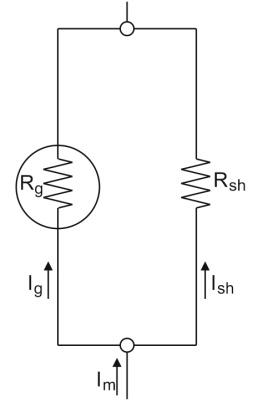
\includegraphics[width=0.3\linewidth]{fig/screenshot002}
	\label{fig:screenshot002}
\end{figure}
		Della $I_m$ totale, si fa passare sul galvanometro la corrente $I_g$ che questo può sopportare mentre il resto scorre sulla resistenza di shunt $R_{sh}$, è ovviamente una corrente di maggiore entità.
		\[I_m = I_g + I_{sh}\]
		\[V = I_gR_g = I_{sh}R_{sh}\Rightarrow I_{sh} = I_g{R_g\over R_{sh}}\]
		Per cui:
		\[I_m = \left(1+{R_g\over R_{sh}}\right)I_g\]
		\textit{Esempio}: con $R_g= 50\Omega, I_g = 1mA$, come deve essere la resistenza di shunt? 
		\[I_m = \left(1+{R_g\over R_{sh}}\right)I_g \Rightarrow R_{sh}I_m = \left(R_{sh}+R_g\right)I_g \Rightarrow R_{sh}I_m = R_{sh}I_g+R_gI_g \] 
		\[R_{sh}(I_m-I_g) = R_gI_g \]
		\[R_{sh} = \dfrac{I_g}{I_m-I_g}R_g\]
		Per cui in questo caso:
		\[R_{sh} = \dfrac{0.001 A}{5 A-0.001 A}50\Omega = 0.01\Omega\]
\end{adjustwidth}
\newpage		
\subsubsection{Amperometro Multicampo}	
\begin{adjustwidth}{2in}{}
		L'amperometro può essere uno strumento multicampo, ovvero tramite uno switch che sceglie la resistenza di shunt da mettere in parallelo, può misurare diverse correnti.
\begin{figure}[H]
	\centering
	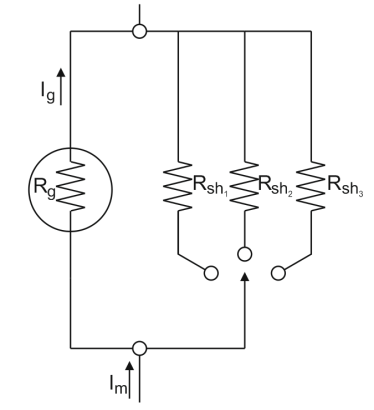
\includegraphics[width=0.3\linewidth]{fig/screenshot003}
	\label{fig:screenshot003}
\end{figure}
		Ad esempio sempre con $R_g= 50\Omega, I_g = 1mA$:
		\[\begin{cases}
			R_{sh}^1=50\Omega \Rightarrow I_m = 2mA \\
			R_{sh}^2=10\Omega \Rightarrow I_m = 6mA \\
			R_{sh}^3=5\Omega \Rightarrow I_m = 11mA \\
		\end{cases}\]
		Ruotando lo switch si cambia il campo di misura, ma per quale necessità? 
		
		Se serve misurare una piccola corrente scegliendo una grande resistenza come può essere il caso in \textbf{esempio} ma mantenendo invariata la resistenza del galvanometro, trovando una piccola resistenza sul ram di shunt la corrente passerà interamente lì col rischio che non percorra il galvanometro, in questo modo facendo passare sul galvanometro una corrente sempre minore si rischia la sottorisoluzione, ovvero la corrente che scorre sullo strumento non basta neanche a far muovere il nucleo ferromagnetico. 
		
		È perciò importante selezionare il campo di misura più adeguato, quello più vicino alla corrente che si intende misurare. \newline 
		
		Tuttavia nè il galvanometro nè l'amperometro riescono a misurare correnti elevate anche mediante l'utilizzo di resistenze molto basse, infatti queste verrebbero facilmente  bruciate.  
\end{adjustwidth}
\newpage		
\subsection{Pinza Amperometrica}	
\begin{adjustwidth}{2in}{}
		Per la misura di correnti elevate e per evitare di mettere in serie l'amperometro o il galvanometro per misurare la corrente e quindi interrompere il circuito, si sceglie la pinza amperometrica. In questo modo, non interferendo minimamente col circuito, presenta un errore di inserzione nullo.  
\begin{figure}[H]
	\centering
	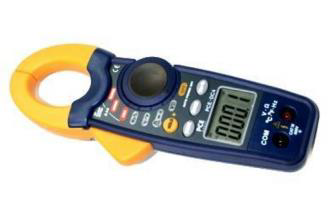
\includegraphics[width=0.3\linewidth]{fig/screenshot004}
	\label{fig:screenshot004}
\end{figure}
		La pinza amperometrica possiede sensori diversi per principi di misure diversi. 
\begin{flushright}
		\begin{table}[H]
			\begin{tabular}{|l|l|lll}
				\cline{1-2}
				Corrente Alternata                                                                                                                                                                                & Corrente continua                                                                                                                                                                                                                                                                                              &  &  &  \\ \cline{1-2}
				Induzione Elettromagnetica                                                                                                                                                                        & Effetto Hall                                                                                                                                                                                                                                                                                                   &  &  &  \\
				\begin{tabular}[c]{@{}l@{}}Un trasformatore attrverso una variazione del \\ $\varphi(\vec{B})$ che determina una corrente\\ sul circuito secondario.\end{tabular} & \begin{tabular}[c]{@{}l@{}}l’effetto Hall, riguarda la formazione di \\ una differenza di potenziale tra le opposte \\ facce di un conduttore elettrico; tale \\ differenza è attribuibile a un campo \\ magnetico che si pone perpendicolarmente \\ rispetto al flusso della corrente elettrica.\end{tabular} &  &  &  \\
				L'elemento ferromagnetico è la pinza                                                                                                                                                              & \begin{tabular}[c]{@{}l@{}}Una corrente genera un campo magnetico \\ che genera uno spostamento di cariche e quindi \\ una variazione di tensione\end{tabular}                                                                                                                                                 &  &  &  \\
				\begin{tabular}[c]{@{}l@{}}Il primario è ad un solo avvolgimento ed è \\ il filo da misurare\end{tabular}                                                                                         &                                                                                                                                                   &  &  &  \\
				\begin{tabular}[c]{@{}l@{}}Il secondario è all'interno dello strumento.\\ Si ottiene una misura dallo strumento\\ poporzionale a quella del pirmario.\end{tabular}                                &                                                                                                                                                                                                                                                                                                                &  &  &  \\
				Non si possono misurare correnti costanti                                                                                                                                                         &                                                                                                                                                                                                                                                                                                                &  &  &  \\ \cline{1-2}
			\end{tabular}
		\end{table}
\end{flushright}
\end{adjustwidth}
\begin{figure}[H]
	\centering
	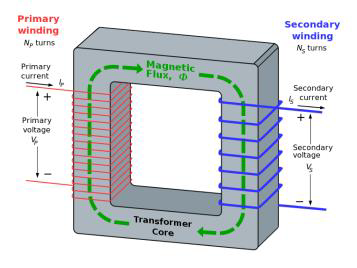
\includegraphics[width=0.3\linewidth]{fig/screenshot005}
	\caption{Ganasce, elemento ferromagnetico}
	\label{fig:screenshot005}
\end{figure}
\begin{figure}[H]
	\centering
	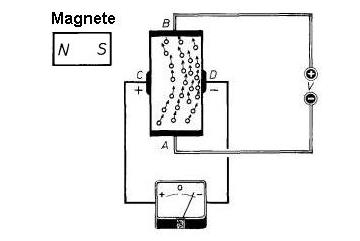
\includegraphics[width=0.3\linewidth]{fig/screenshot006}
	\caption{Effetto Hall}
	\label{fig:screenshot006}
\end{figure}
		Con la pinza amperometrica si riescono a misurare correnti elevate, anche dell'ordine delle 600A.  
\newpage		
\section{Misure di tensione}
\subsection{Voltmetro}	
\begin{adjustwidth}{2in}{}		
		La misura di tensione avviene in parallelo al circuito, lo strumento è sempre costituito da un galvanometro in serie ad una resistenza di shunt $R_v$ ora in serie al galvanometro.
\begin{figure}[H]
	\centering
	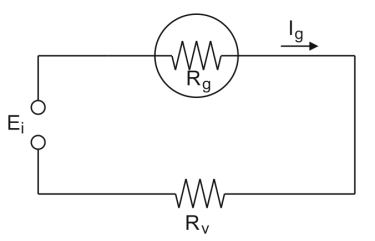
\includegraphics[width=0.3\linewidth]{fig/screenshot007}

	\label{fig:screenshot007}
\end{figure}
		\[E_i = I_g(R_v + R_g)\]		
		L'errore di inserzione per le misure di tensione è:
		\[\varepsilon_{ins} = \dfrac{R_{\text{ingresso/sensore}}}{R_{\text{misuratore}}}\]
		Per cui essendo la resistenza del galvanometro molto bassa, si dovrà avere una resistenza di shunt elevata. 
		\[R_v = {E_i\over I_g} - R_g\]
		Un'elevata resistenza del voltmetro diminuirà l'errore di inserzione. 
\end{adjustwidth}
%\newpage		
\subsubsection{Voltmetro Multicampo}	
\begin{adjustwidth}{2in}{}			
		Il voltmetro multicampo, analogamente all'amperometro, ha una serie di switch che permettono la scelta della resistenza ora da mettere in sere al galvanometro.		
		\begin{figure}[H]
			\centering
			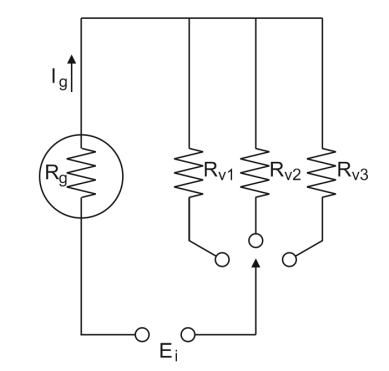
\includegraphics[width=0.3\linewidth]{fig/screenshot008}
			\label{fig:screenshot008}
		\end{figure}		
		Ad esempio per misurare una tensione $E_i = 100 mV$ avendo un galvanometro da $R_g = 30\Omega$ e $I_g = 20\mu A$ si sceglie una resistenza di shunt pari a:
		\[R_v = {0.1V\over 0.00002A} - 30\Omega = 4970\Omega\]
		Si possono realizzare voltmetri multicampo che vadano dai 100mV ai 1000V. \newline 
		
		Voltmetro e amperometro sono concettualmente identici e sono entrambi strumenti passivi.  
\end{adjustwidth}
%\newpage		
\subsection{Voltmetro Potenziometrico}	
\begin{adjustwidth}{2in}{}		
		Il voltmetro potenziometrico è uno strumento di zero, indicherà perciò l'equilibrio.
		
		Si confronterà perciò una tensione di riferimento nota $E_R$, tensione di alimentazione del potenziometro, con la tensione data dallo scorrimento di un palpatore sul potenziometro, indicando dove questa raggiunge lo zero. 
		
		\[\boxed{\text{potenziometro}}\leftarrow \boxed{\text{palpatore}} \leftarrow \boxed{\text{galvanometro}}\]
\begin{figure}[H]
	\centering
	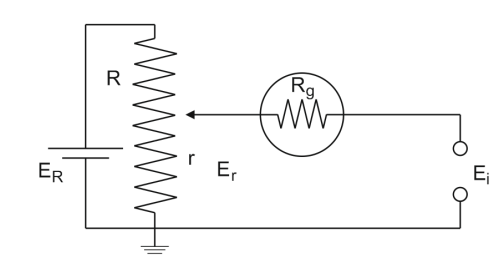
\includegraphics[width=0.5\linewidth]{fig/screenshot009}
	\label{fig:screenshot009}
\end{figure}
		\[r = [0, R] \hspace{1cm} E_r = [0, E_R]\]
		\[E_R = IR \hspace{1cm} E_r = Ir\]
		\[E_r = {r\over R}E_R\]

		Si vuole che l'indicatore dello strumento segni lo zero. 
		
		La scala graduata, indicando la porzione di resistenza presa in esame, indica la tensione che si sta misurando: Se $ E_i \ne E_r $ nel galvanometro passa corrente, per cui la misura di zero si avrà quando:
		\[E_i = E_r = {r\over R}E_R\]  
		Anche in questo caso si hanno errori di inserzione nulli dovuti al semplice fatto che lo strumento è semplicemente utilizzato per verificare la condizione $I_g = 0$: quando non passa corrente si hanno tensioni uguali e si misura lo zero. \newline 
		
		È uno strumento attivo, dato che necessita di alimentazione, ed è usato per la sola misurazione di corrente statica, non tempo variante.
\end{adjustwidth}
\newpage		
\subsection{Voltmetro Digitale}	
\begin{adjustwidth}{2in}{}	
		Rispetto ad un voltmetro analogico, quello digitale garantisce tre vantaggi, come maggiore precisione, maggiore velocità di lettura e un limitato livello di rumore. 		 
		\begin{figure}[H]
			\centering
			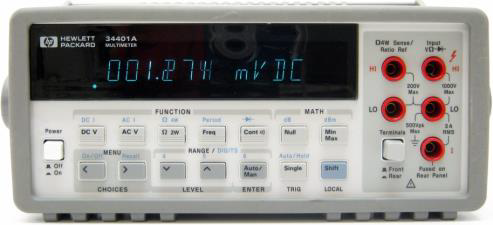
\includegraphics[width=0.5\linewidth]{fig/screenshot010}
			\label{fig:screenshot010}
		\end{figure}		
		Il risultato è presente su di un display con un'incertezza di tipo uniforme, dalla distribuzione rettangolare. 
		
		All'interno alloggerà un convertitore da analogico a digitale A/D, ed è nient'altro che un multimetro, fornendo la possibilità quindi di misurare sia corrente che tensione che resistenza. \newline 
		
		Un voltmetro digitale garantisce inoltre una certa \textbf{sovraportata}, riuscendo quindi a misurare - per una certa percentuale del fondo scala - grandezze maggiori del suo campo di misura. 
		
		Il display permette poi la visualizzazione di un certo \textbf{numero di digit}. Ad esempio con 3 digit lo strumento permette la visualizzazione di numeri da 999 a 0,00. La scelta di dove porre la virgola mobile sarà poi dipendente dallo sperimentatore e dalla risoluzione che si vuole ottenere, prestando attenzione a non perdere informazioni: 1,2 è un'informazione molto meno dettagliata di 1,23.
		
		Può essere poi presente un "mezzo" digit che può assumere solo il valore di 0 o 1, in questo caso possono essere rappresentati numeri da 1999 a 0,000 con una sovraportata del 100\%. 
		
		La \textbf{portata} del voltmetro digitale rappresenta il range di misura del voltmetro in funzione delle cifre a
		disposizione. La portata può essere fatta variare spostando la virgola. Sono
		permesse misure tra 0,000 e 1,999; 00,00 e 19,99; 000,0 e 199,9; 0000 e 1999.
		L’aumento del fondo scala determina naturalmente un aumento dell’incertezza.
		
		Il \textbf{tempo di misura} è semplicemente il tempo necessario allo strumento per effettuare la misurazione.  
\end{adjustwidth}
\newpage
\section{Misure di Resistenza}	
\subsection{Ponte di Wheatstone}	
\begin{adjustwidth}{2in}{}
		Da un punto di vista strettamente sperimentale, lo scopo di una misura non è quello di determinare l'esatto valore di una grandezza ma piuttosto individuare un idoneo intervallo che contenga tale grandezza con una probabilità ragionevole.
		Misurare una resistenza può apparire un'operazione semplice e alla portata di tutti... "basta avere un tester con adeguato fondo scala" ma in realtà è così solo se si prescinde dalla precisione e dall'accuratezza con cui vogliamo ottenere il risultato.
		
		La teoria e la pratica delle misure elettriche ci insegnano che esistono diversi metodi per misurare una resistenza i quali vanno applicati in base all'ordine di grandezza e alla precisione che si desidera ottenere.
		Il primo e il più conosciuto è senz'altro il metodo volt-amperometrico che consente di determinare il valore di una resistenza alimentata con un'opportuna tensione continua Vcc, misurando tensione e corrente e facendone poi il rapporto. La precisione della misura in questo caso dipende solo dalla qualità e dalla corretta calibrazione della strumentazione di misura utilizzata (un voltmetro e un amperometro) e normalmente consente di soddisfare la maggior parte delle esigenze pratiche.\newline
		
		In tutti quei casi in cui occorra invece misurare una resistenza con una precisione superiore a quella fornita dal metodo volt-amperometrico si può utilizzare un metodo di misura che adotta uno schema circuitale detto \textbf{ponte di Wheatstone}.\newline 
		
		Il ponte di Wheatstone è costituito da quattro rami ciascuno contenente una resistenza, un elemento passivo, al cui interno è posto un rilevatore, che sia un amperometro (galvanometro + shunt in parallelo) o voltmetro (galvanometro + shunt in serie).
\begin{figure}[H]
	\centering
	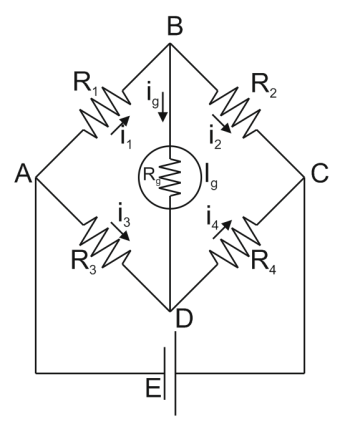
\includegraphics[width=0.2\linewidth]{fig/screenshot011}
	\label{fig:screenshot011}
\end{figure}
		Esso viene normalmente alimentato per mezzo di un generatore di tensione costante $E$ ed è utilizzato allo scopo di determinare il valore incognito di una delle quattro resistenze.\newline 
		
		Questo strumento permette due possibili misure: quella di zero, per ingresso statico; e quella di deflessione. 
\end{adjustwidth}
\newpage
\subsubsection{Metodo di zero}	
\begin{adjustwidth}{2in}{}
		Lo strumento rilevatore è un amperometro e segnerà l'equilibrio quando $I_g =0$. 		
\begin{figure}[H]
	\centering
	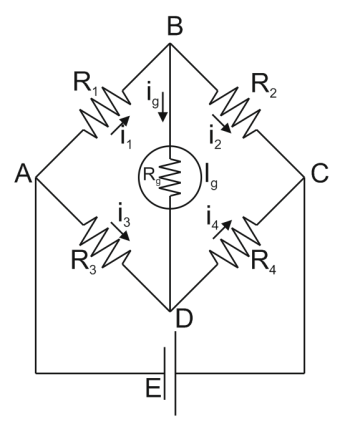
\includegraphics[width=0.3\linewidth]{fig/screenshot011}
	\label{fig:screenshot011.2}
\end{figure}		
		Si pone come resistenza da misurare $R_1, R_2, R_4$ sono resistenze note, mentre $R_3\nearrow$ è una resistenza variabile, un potenziometro, Sarà questa infatti a variare fino a quando si misurerà una corrente nulla sul galvanometro, ma come si arriva a questa condizione? L'unica condizione che soddisfa una corrente nulla sul galvanometro è:
		\[I_g = 0 \Rightarrow E_g = 0 \Leftrightarrow V_D = V_B\]
		Da questo risultato, si sottrae in due casi la stessa quantità, prima $V_A$ e poi $V_C$:
		\[V_B = V_D\]
		\[\begin{cases}
			V_B - V_A = V_D - V_A \\
			V_B - V_C = V_D - V_C \Leftrightarrow V_C - V_B = V_C - V_D
		\end{cases}
		\]
		A queste differenze di potenziale corrispondono rispettivamente:
		\[\begin{cases}
			I_1R_1 = I_3R_3 \\
			I_2R_2 = I_4R_4
		\end{cases}
		\]
		Dividendo membro si ottiene:
		\[\dfrac{I_1R_1}{I_2R_2} = \dfrac{I_3R_3}{I_4R_4}\]
		Dall'equilibrio delle correnti al nodo $B$ si ottiene: \(I_1 - \cancel{I_g} - I_2 = 0 \Rightarrow I_1 = I_2\) così come \(I_3 = I_4\), allora: 
		\[\dfrac{R_1}{R_2} = \dfrac{R_3}{R_4}\]
		Avendo la libertà di scegliere, essendo queste note, \(R_2 = R_4\) ci si riconduce a:
		\[ R_1 = R_3\]
		Quando la resistenza individuata sul potenziamento è uguale alla resistenza incognita $ R_1 $, si arresta il flusso di corrente $ I_g  $e si misurerà conseguentemente con precisione la resistenza incognita. \newline 
		
		Inutilizzabile se $R_1$ varia nel tempo, si dovrebbe rincorrere la resistenza variabile sul potenziometro.  
\end{adjustwidth}
\newpage
\subsubsection{Metodo a deflessione - Voltmetro}	
\begin{adjustwidth}{2in}{}	
		Il metodo a deflessione è usato per misure dinamiche poco variabili e permette di leggere un'uscita su di una scala graduata in base alla corrente e alla tensione che interessano la resistenza incognita. \newline
		
		Nel metodo a deflessione si possono usare come strumenti rivelatori o un voltmetro $R_{\text{strumento}}\rightarrow\infty \Rightarrow I_g\rightarrow0$, o un amperometro $R_g\ne0\Rightarrow I_g\ne0$ d'altra parte è la corrente che serve per misurare. 
		
\paragraph{Voltmetro} \mbox{} \\		
		\begin{figure}[H]
			\centering
			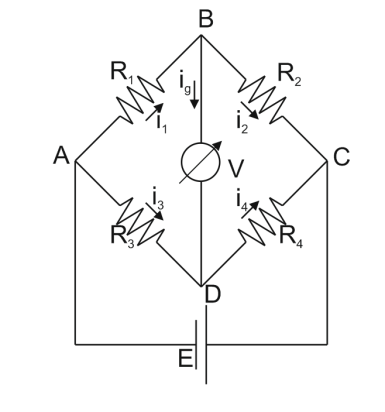
\includegraphics[width=0.3\linewidth]{fig/screenshot012}
			\label{fig:screenshot012}
		\end{figure}
		Per l'equilibrio ai nodi $B$ e $D$ e dato che $I_g=0$:
		\[I_1 = I_2 \hspace{1cm} I_3 = I_4\]
		Maglia ABD:
		\[V = I_1R_1 - I_3R_3\]
		Maglia BCD:
		\[V = I_2R_2-I_4R_4 = I_1R_2-I_3R_4\]
		La misura del voltmetro dovrà essere la stessa, per cui
		\[ V = I_1R_1 - I_3R_3 = I_1R_2-I_3R_4 \]
		Maglia ABC:
		\[E = R_1I_1+R_2I_2 = I_1(R_1+R_2)\]
		Maglia ADC:
		\[E = I_3R_3+I_4R_4 = I_3(R_3+R_4)\]
		Essendo la tensione di alimentazione la stessa:
		\[E = I_1(R_1+R_2) = I_3(R_3+R_4)\]
		Ottenendo un sistema descritto dalle incognite $I_3, I_4$:
		\[\begin{cases}
			I_1R_1 - I_3R_3 = I_1R_2-I_3R_4 \\
			I_1(R_1+R_2) = I_3(R_3+R_4)
		\end{cases}\]
		Che risolto conduce a:
		\[I_1 = \dfrac{E}{R_1+R_2}\hspace{1cm}I_3 = \dfrac{E}{R_3+R_4}\]
		Che sostituite in \(V = I_1R_1 - I_3R_3\) conducono a:
		\[V = E\left(\dfrac{R_1}{R_1+R_2} - \dfrac{R_3}{R_3+R_4} \right) = E\left[\dfrac{R_1R_4-R_2R_3}{(R_1+R_2)(R_3+R_4)}\right]\]
		Quando il ponte è bilanciato l'uscita dello strumento rivelatore è nulla:
		\[ V = E\left[\dfrac{R_1R_4-R_2R_3}{(R_1+R_2)(R_3+R_4)}\right] = 0 \Leftrightarrow R_1R_4=R_2R_3 \]
		
		E se la resistenza da misurare fosse variabile, come varierebbe l'uscita del voltmetro? 
		
\paragraph{Configurazione a quarto di ponte} \mbox{} \\		
		\textbf{Variazione di una sola resistenza.}		
		\begin{figure}[H]
			\centering
			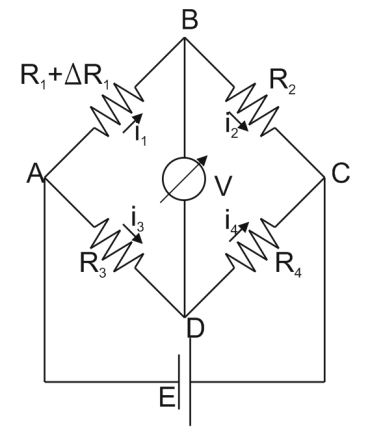
\includegraphics[width=0.3\linewidth]{fig/screenshot013}
			\label{fig:screenshot013}
		\end{figure}				
		In che modo varia $\Delta V$ variando $\Delta R$?
		\[R_1 = R_1 + \Delta R_1\]
		\[V+\Delta V = E\left[\dfrac{(R_1+ \Delta R_1)R_4-R_2R_3}{(R_1+ \Delta R_1+R_2)(R_3+R_4)}\right]\]
		Sotto l'ipotesi di resistenze uguali: $R_1=R_2=R_3=R_4=R\Rightarrow V=0$ rimarrà quindi il solo termine:
		\[\Delta V = E\left(\dfrac{R\Delta R}{4R^2 + 2R\Delta R}\right)\]
		Normalizzando: 
		\[\dfrac{\Delta V}{E} = \dfrac{\nicefrac{\Delta R}{R}}{4+2\nicefrac{\Delta R}{R}}\]
		Basterà quindi misurare un $\Delta V$ per ottenere un $\Delta R$. \newline 
		
		L'andamento dell'equazione trovata è lineare? No, è come se fosse 
		 \[y = \dfrac{x}{A+x}\]		
		\begin{itemize}
		\item Per \(\dfrac{\Delta R}{R}\rightarrow0 ~ \dfrac{\Delta V}{E} \rightarrow 0\)
		
		\item Per \(\dfrac{\Delta R}{R}\rightarrow+\infty ~ \dfrac{\Delta V}{E} \rightarrow {1\over2}\) 
		
		\item Per \(\dfrac{\Delta R}{R}\rightarrow-\infty ~ \dfrac{\Delta V}{E} \rightarrow -2\)	
		\end{itemize}	
		\begin{figure}[H]
			\centering
			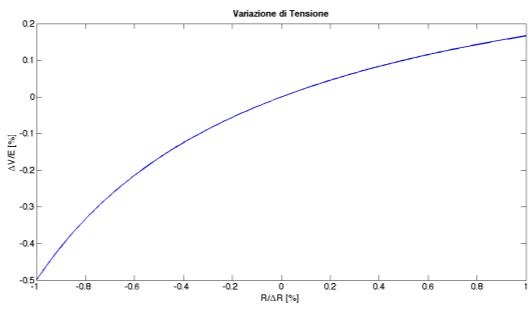
\includegraphics[width=0.5\linewidth]{fig/screenshot014}
			\label{fig:screenshot014}
		\end{figure}		
		Dato che si spinge per avere una sensibilità sempre costante su tutto il campo di misura, si mira ad avere una funzione caratteristica che sia lineare, ma questa non lo è.
		
		Si restringe quindi il campo di misura a $\Delta R$ piccoli, in questo modo la funzione la si osserva essere lineare e diviene: 
		\[\dfrac{\Delta V}{E} = {1\over4}\dfrac{\Delta R}{R}\]
		Ottenendo un $\Delta V$ chiaramente proporzionale al $\Delta R$.		
		\begin{figure}[H]
			\centering
			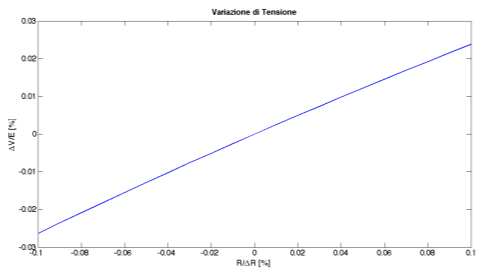
\includegraphics[width=0.5\linewidth]{fig/screenshot015}
			\label{fig:screenshot015}
		\end{figure}				
		Siccome però non ha senso fisico considerare resistenze negative, l'unico grafico che si considererà sarà solo nel semipiano positivo.  

\paragraph{Configurazione a mezzo ponte I} \mbox{} \\				
		\textbf{Variazione di due resistenze opposte $R_1, R_4$}		
		\begin{figure}[H]
			\centering
			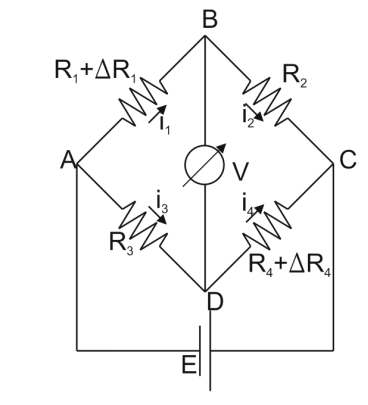
\includegraphics[width=0.3\linewidth]{fig/screenshot016}
			\label{fig:screenshot016}
		\end{figure}				
		\[R_1 = R_1 + \Delta R_1 \hspace{1cm} R_4 = R_4 + \Delta R_4 \]
		\[V+\Delta V = E\left[\dfrac{(R_1+ \Delta R_1)(R_4 + \Delta R_4)-R_2R_3}{(R_1+ \Delta R_1+R_2)(R_3+R_4 + \Delta R_4)}\right]\]
		Sotto l'ipotesi di resistenze uguali: $R_1=R_2=R_3=R_4=R\Rightarrow V=0$ rimarrà quindi il solo termine:
		\[\Delta V = E\left(\dfrac{R\Delta R_1 + R\Delta R_4 + \Delta R_1\Delta R_4 }{4R^2 + 2R\Delta R_1+2R\Delta R_4 + \Delta R_1\Delta R_4}\right)\]
		Normalizzando: 
		\[\dfrac{\Delta V}{E} = \dfrac{\nicefrac{\Delta R_1}{R} + \nicefrac{\Delta R_4}{R} + \nicefrac{(\Delta R_1\Delta R_4)}{R^2}}{4+2\nicefrac{\Delta R_1}{R} + 2\nicefrac{\Delta R_4}{R} + \nicefrac{(\Delta R_1\Delta R_4)}{R^2}}\]
		Per $\Delta R$ piccoli:
		\[\dfrac{\Delta V}{E} = {1\over4}\left(\dfrac{\Delta R_1}{R} + \dfrac{\Delta R_4}{R}\right)\]
		Ottenendo anche il grande risultato che le variazioni di resistenza su rami opposti si sommano. 
		
		Se poi si fa in modo che le variazioni delle due resistenze misurate siano uguali, ovvero $\Delta R_1 = \Delta R_4 = \Delta R$, si ottiene:
		\[\dfrac{\Delta V}{E} = {1\over2}\dfrac{\Delta R}{R}\]
		Ed una sensibilità raddoppiata.  
		
		\paragraph{Configurazione a mezzo ponte II} \mbox{} \\
		\textbf{Variazione di due resistenze contigue $R_1, R_2$}
			\begin{figure}[H]
				\centering
				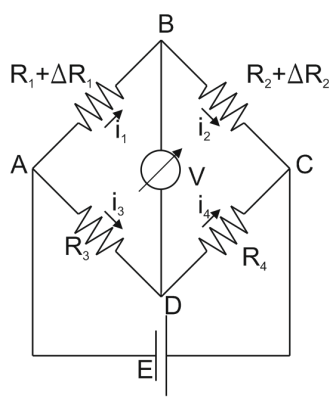
\includegraphics[width=0.3\linewidth]{fig/screenshot017}
				\label{fig:screenshot017}
			\end{figure}				
		\[R_1 = R_1 + \Delta R_1 \hspace{1cm} R_2 = R_2 + \Delta R_2 \]
		\[V+\Delta V = E\left[\dfrac{(R_1+ \Delta R_1)R_4-(R_2 + \Delta R_2)R_3}{(R_1+ \Delta R_1+R_2 + \Delta R_2)(R_3+R_4)}\right]\]
		Sotto l'ipotesi di resistenze uguali: $R_1=R_2=R_3=R_4=R\Rightarrow V=0$ rimarrà quindi il solo termine:
		\[\Delta V = E\left(\dfrac{R\Delta R_1 - R\Delta R_2}{4R^2 + 2R\Delta R_1+2R\Delta R_2}\right)\]
		Normalizzando: 
		\[\dfrac{\Delta V}{E} = \dfrac{\nicefrac{\Delta R_1}{R} - \nicefrac{\Delta R_2}{R}}{4+2\nicefrac{\Delta R_1}{R} + 2\nicefrac{\Delta R_2}{R}}\]
		Per $\Delta R$ piccoli:
		\[\dfrac{\Delta V}{E} = {1\over4}\left(\dfrac{\Delta R_1}{R} - \dfrac{\Delta R_2}{R}\right)\]
		Ottenendo anche il grande risultato che le variazioni di resistenza su rami contigui si sottraggono. 
		
		Se poi si fa in modo che le variazioni delle due resistenze misurate siano uguali, ovvero $\Delta R_1 = \Delta R_2 = \Delta R$, si ottiene:
		\[\dfrac{\Delta V}{E} = 0\]
		Ossia un annullamento della sensibilità. 
\newpage		
\paragraph{Configurazione a ponte intero} \mbox{} \\
		\begin{figure}[H]
			\centering
			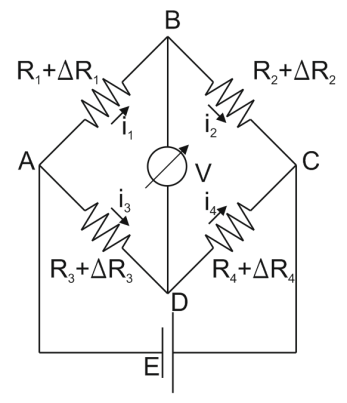
\includegraphics[width=0.3\linewidth]{fig/screenshot018}
			\label{fig:screenshot018}
		\end{figure}
		\[R_1 = R_1 + \Delta R_1 \hspace{1cm} R_2 = R_2 + \Delta R_2 \]
		\[R_3 = R_3 + \Delta R_3 \hspace{1cm} R_4 = R_4 + \Delta R_4 \]
		\[V+\Delta V = E\left[\dfrac{(R_1+ \Delta R_1)(R_4 + \Delta R_4)-(R_2 + \Delta R_2)(R_3 + \Delta R_3)}{(R_1+ \Delta R_1+R_2 + \Delta R_2)(R_3 + \Delta R_3+ R_4 + \Delta R_4)}\right]\]
		Sotto l'ipotesi di resistenze uguali: $R_1=R_2=R_3=R_4=R\Rightarrow V=0$ rimarrà quindi il solo termine che normalizzato e per $\Delta R$ piccoli diviene:
		\[\dfrac{\Delta V}{E} = {1\over4}\left(\dfrac{\Delta R_1}{R} - \dfrac{\Delta R_2}{R} - \dfrac{\Delta R_3}{R} + \dfrac{\Delta R_4}{R}\right)\]
		Si distinguano due casi:
		\begin{enumerate}
			\item Se $\Delta R_1 = \Delta R_2 = \Delta R_3 = \Delta R_4 = \Delta R$ e quindi si fa in modo che le variazioni resistenza siano uguali su tutti i rami, si ottiene:
			\[\dfrac{\Delta V}{E} = 0\]
			Ossia un annullamento della sensibilità.
			
			\item Se $\Delta R_1 = -\Delta R_2 = -\Delta R_3 = \Delta R_4 = \Delta R$ e quindi si fa in modo che le variazioni resistenza siano uguali in modulo su tutti i rami ma opposte su rami opposti e quindi diverse su rami contigui, si ottiene:
			\[\dfrac{\Delta V}{E} = \dfrac{\Delta R}{R}\]
			Ossia una sensibilità quadruplicata: Si misura un $\Delta V$ grazie ad una variazione di resistenza $\Delta R$			
		\end{enumerate}
\newpage
		\paragraph{Esempio: lamina incastrata e cella di carico}\mbox{} \\ 
		\begin{figure}[H]
			\centering
			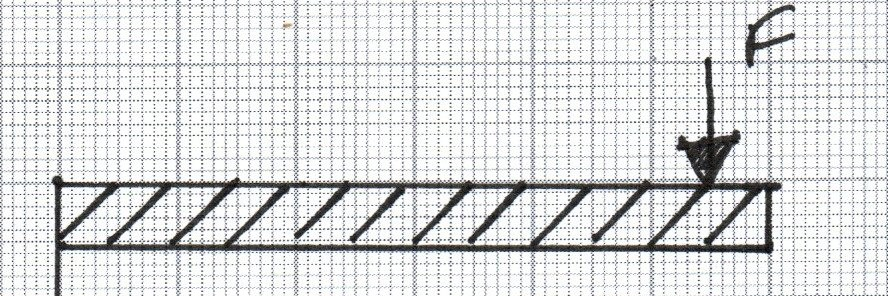
\includegraphics[width=0.3\linewidth]{fig/mm_1}
			\label{fig:mm1}
		\end{figure}

		Si immagini di porre solo due estensimetri A e B sul lato superiore della barra incastrata, in questo modo tuttavia si ottiene una sensibilità minore del caso di 4 estensimetri. 		
\begin{figure}[H]
	\centering
	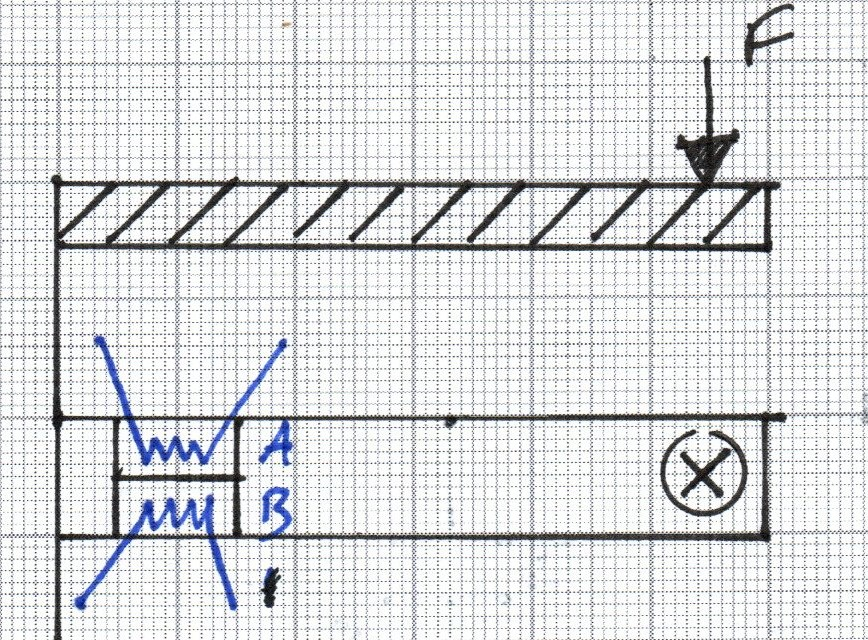
\includegraphics[width=0.3\linewidth]{fig/mm_2}
	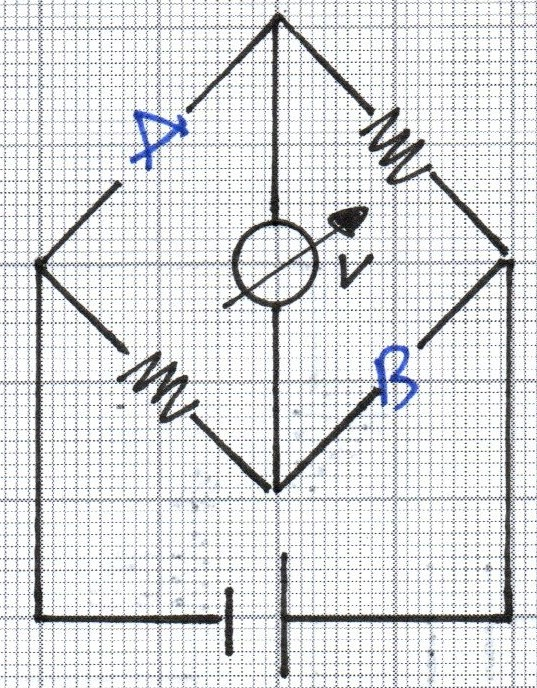
\includegraphics[width=0.2\linewidth]{fig/mm_4}
\end{figure}
		Si rimedia quindi ponendo due estensimetri C e D anche sotto alla barra incastrata, negli stessi punti dove sono stati applicati gli altri estensimetri, ma in modo da misurare una variazione di resistenza opposta a quelli del lato superiore. Si noti inoltre come non abbia la minima importanza la maniera con cui si collegano C e D ai rami A e B, l'importante è che risultino opposti e misurino in modulo le stesse deformazioni.  
\begin{figure}[H]
			\centering
			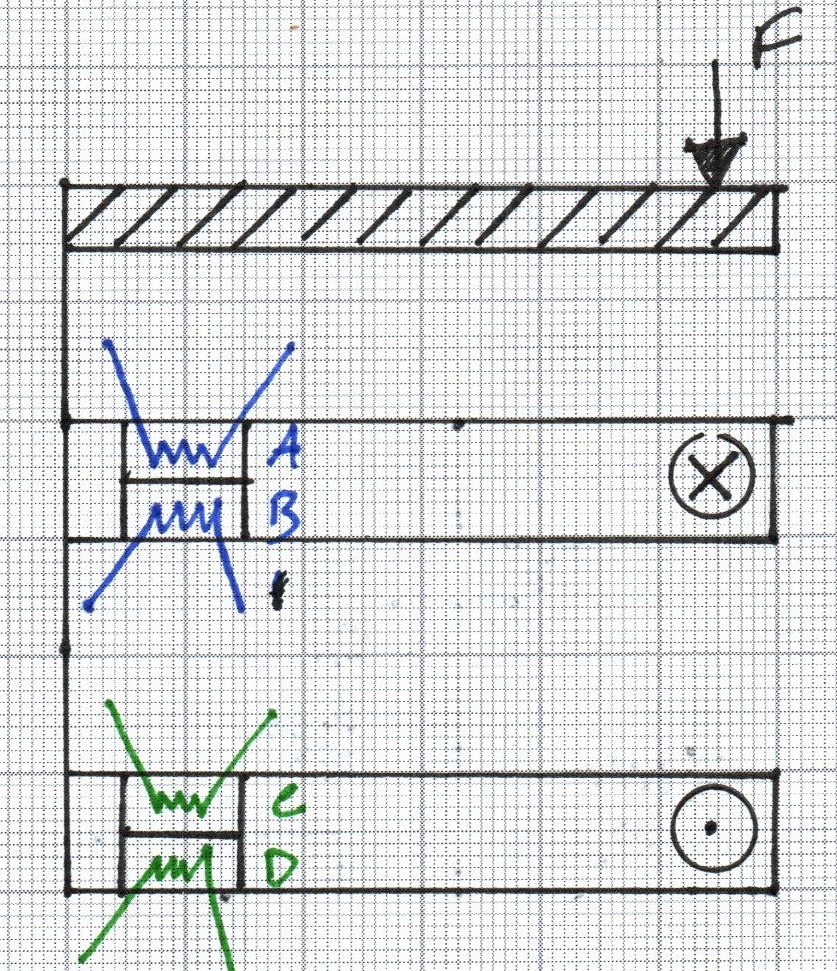
\includegraphics[width=0.3\linewidth]{fig/mm_3}
			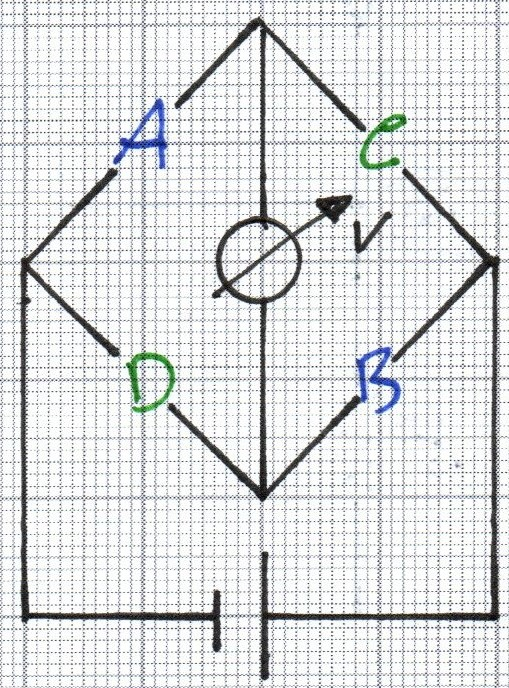
\includegraphics[width=0.2\linewidth]{fig/mm_5}
\end{figure}
\end{adjustwidth}
\newpage
\subsubsection{Metodo a deflessione - Amperometro}	
\begin{adjustwidth}{2in}{}		
		A differenza del metodo a deflessione con il voltmetro qui $R_g\downarrow$, deve scorrere una corrente $I_g$ che lo strumento rivelatore dovrà misurare. 		
		\begin{figure}[H]
			\centering
			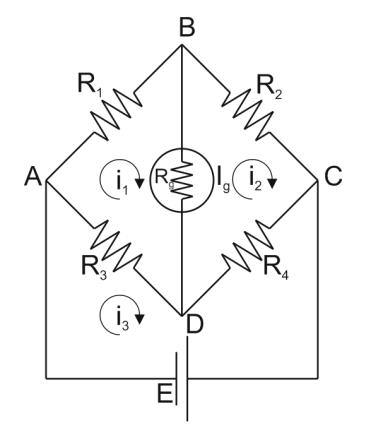
\includegraphics[width=0.3\linewidth]{fig/screenshot019}
			\label{fig:screenshot019}
		\end{figure}
		Per le equazioni delle correnti nelle tre maglie si ottiene:		
		\begin{itemize}
		\item Maglia ABD:
		\[R_1I_1 + R_g(I_1-I_2) + R_3(I_1-I_3) = 0\]
		\item Maglia BCD:
		\[R_2I_2+R_4(I_2-I_3) + R_g(I_2-I_1) = 0\]
		\item Maglia ADC:
		\[R_3(I_3-I_1) + R_4(I_3-I_2) = E\]
		\end{itemize}
		Sul ramo dell'amperometro di legge che la corrente di lato misurata è pari a:
		\[I_g = I_1 - I_2\]
		Le equazioni delle maglie possono essere arrangiate in un sistema: 		
		\[\left\{ \begin{array}{cccc}		
		I_1(R_1 + R_g + R_3) &- I_2R_g  			    &- I_3R_3       &= 0\\
		-I_1R_g  			 &+ I_2(R_2 + R_4 + R_g) &- I_3R_4       &= 0\\
		-I_3R_3  			 &- I_2R_4               &+ I_3(R_3+R_4) &= E	
		\end{array} \right.
		\]
		Che in forma matriciale diviene:
		\[\left[\begin{array}{ccc}
			(R_1+R_g+R_3) & -R_g & -R_3 \\
			-R_g & (R_3+R_4+R_g) & -R_4 \\
			-R_3 & -R_4 & (R_3+R_4)
		\end{array}\right]\left[\begin{array}{c}
		I_1 \\
		I_2 \\
		I_3
		\end{array}\right] = \left[\begin{array}{c}
		0 \\
		0 \\
		E
		\end{array}\right]\]
		Trovando $I_1, I_2$, si sostituiscono in $I_g$ e portano a
		\[I_g = E\dfrac{R_1R_4-R_2R_3}{R_g[(R_1+R_2)(R_3+R_4)] + R_1R_2(R_3+R_4) + R_3R_4(R_1+R_2)}\]		
		Per cui	considerando una resistenza variabile ed una configurazione a quarto di ponte: 
		\[R_1 = R_1 + \Delta R_1 \]
		Con l'ipotesi di $R_1=R_2=R_3=R_4=R\Rightarrow I_g=0$ e rimane soltanto:
		\[\Delta I_g = \dfrac{E}{R}\dfrac{\nicefrac{\Delta R}{R}}{\nicefrac{R_g}{R}\left(4+2\nicefrac{\Delta R}{R}\right) + 4 + 3\nicefrac{\Delta R}{R}}\]
		Per $R_g\rightarrow0$, d'altronde si deve garantire una lettura sull'amperometro:
		\[\dfrac{\Delta I_g}{\nicefrac{E}{R}} = \dfrac{\nicefrac{\Delta R}{R}}{4 + 3\nicefrac{\Delta R}{R}}\]
		Per $ \Delta R $ piccoli:
		\[\dfrac{\Delta I_g}{\nicefrac{E}{R}} = \dfrac{\Delta R}{4R}\]
		Evidenziando un andamento lineare.  
		
\paragraph{Nota Bene}\mbox{} \\ 		
		Dato che l'approccio al ponte di Wheatstone col metodo a deflessione utilizzando l'amperometro è concettualmente simile a quello effettuato con il voltmetro, valgono le stesse considerazioni fatte col voltmetro, per cui:
		\begin{itemize}
			\item Variazioni di resistenza su rami opposti si sommano;
			
			\item Variazioni di resistenza su rami contigui si sottraggono;
			
			\item La sensibilità si annulla se c’è una stessa variazione di resistenza sui rami contigui;
			
			\item La sensibilità si annulla se c’è una stessa variazione di resistenza su tutti i rami;
			
			\item La sensibilità raddoppia se c’è una stessa variazione di resistenza sui rami opposti;
			
			\item La sensibilità quadruplica se c’è una stessa variazione di resistenza sui rami opposti
			e di segno opposto sui rami contigui.
		\end{itemize}
\end{adjustwidth}
%\newpage
\subsubsection{Limitazioni}	
\begin{adjustwidth}{2in}{}
		Il ponte di Wheatstone presenta tuttavia delle limitazioni, ad esempio i cavi di collegamento in materiale metallico - dotati di resistenze proprie, possono influenzare  le piccole variazioni di resistenza che si devono misurare, col metodo di zero si dovrebbe misurare uno zero ma nella realtà dei fatti si misura un offset, una sovrastima. 
		
		Il problema potrebbe essere eliminato utilizzando cavi uguali su rami contigui in modo  che le variazioni di resistenza proprie dei cavi di collegamento si eliminino, ma non è sempre banale ottenere cavi di collegamento dalle resistenze perfettamente identiche; un altro modo per correggere la misura potrebbe essere quello di misurare a priori la resistenza dei cavi di collegamento e sottrarla alla misura, trattandola come un errore sistematico; oppure ancora si potrebbe effettuare una seconda misura,  invertendo i cavi e mediando i risultati ottenuti. \newline 
		
		Ancor più della presenza di una resistenza non voluta però, spaventa l'effetto termoelettrico: lo scorrimento di corrente in un sistema attivo porta inevitabilmente all'effetto Joule, con conseguente aumento di resistenza data da un aumento di resistività. 
		
		Si approcciano perciò, per evitare errori di misura, diverse tecniche di misurazione. 
\newpage 		
\paragraph{Misura tramite multimetro}
\subparagraph{Metodo a due fili} \mbox{} 
		\begin{figure}[H]
			\centering
			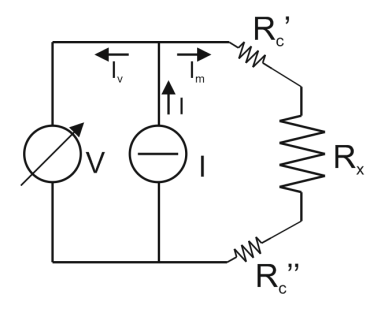
\includegraphics[width=0.3\linewidth]{fig/screenshot020}
			\label{fig:screenshot020}
		\end{figure}
		La misura a due fili è la classica misura effettuata col multimetro, questo infatti, essendo dotato di un proprio generatore interno, forza una intensità di corrente nella resistenza in esame e ne misura la caduta di tensione.
		
		$I_V\downarrow R_V\uparrow$, c'è solo la corrente del multimetro $I_m$ che circola:
		\[V_m = I_mR_x+I_mR'_c+I_mR''_c\]
		Considerando e approssimando i cavi uguali si può trattare l'errore sulla misura della resistenza che ne consegue come un errore sistematico:
		\[\varepsilon=2I_mR_c\]
		Se l'oggetto della misurazione sono resistenze nominalmente elevate, quelle dei due cavi so possono trascurare, come ad esempio si vedrà nelle misure col termistore: $1\Omega$ di cavo rispetto ai $1000\Omega$ della misura non dà effetto. \newline 
		
		Il problema reale sussiste con l'effetto Joule, possono svilupparsi infatti, anche in cavi nominalmente uguali, diversi gradienti di temperatura che non possono essere nè evitati, nè controllati non permettendo l'esatta correzione dell'errore sistematico.  
		
		\subparagraph{Metodo a tre fili} \mbox{} \\
		\begin{figure}[H]
			\centering
			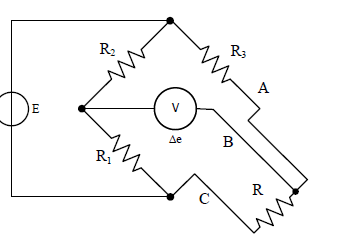
\includegraphics[width=0.5\linewidth]{fig/screenshot021}
			\label{fig:screenshot021}
		\end{figure}
		Un esempio di misura a tre fili avviene con l'estensimetro. \newline 
		
		Si realizza un nodo del ponte di Wheatstone in prossimità della resistenza da misurare, ma se il fine è quello di ottenere una resistenza da misurare minore, un cavo in più non la aumenta? Il cavo che si introduce è collegato al voltmetro, essendo il voltmetro in ogni caso (sia col metodo zero che a deflessione) caratterizzato ad una resistenza/impedenza elevata, in quel cavo non scorre corrente, in più applicando i restati due cavi come in A e C contigui, le due variazioni di resistenza che si vanno a creare si sottraggono ed il loro effetto sulla misurazione si annulla.  
\newpage		
		\subparagraph{Metodo a quattro fili} \mbox{} \\
		\begin{figure}[H]
			\centering
			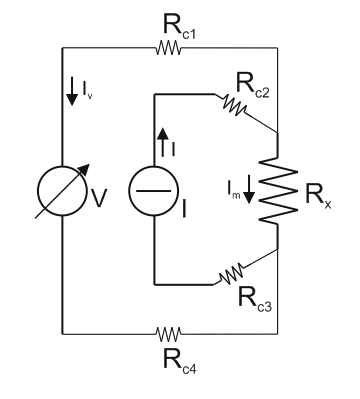
\includegraphics[width=0.3\linewidth]{fig/screenshot022}
			\label{fig:screenshot022}
		\end{figure}
		Il circuito di alimentazione è identificato da una maglia diversa rispetto a quella con cui si fa la misurazione. Di fatto, la maglia di alimentazione non è importante ai fini misuristici perché le sue cadute di tensione su $ R_{c3}, R_{c2} $ non intervengono nella misura, perciò si trascura a piè pari, si ignora: la misura che si vuole ottenere è identificata solamente dalla maglia esterna. \newline 
		
		Il voltmetro infatti misura:
		\[V=I_mR_x+I_vR_{c1} + I_vR_{c4}\]
		Poiché per definizione di multimetro $I_v\ll I_m$ il voltmetro misurerà infine: 
		\[V=I_mR_x+\cancel{I_vR_{c1}} +\cancel{ I_vR_{c4}} \Rightarrow V=I_mR_x\]
		Si ottiene in questo modo un errore sistematico assai trascurabile. \newline 
		
		Questo è un metodo utilizzato per misurare resistenze nominalmente molto basse: due resistenze non entrano in gioco mentre sulle altre due scorre una corrente $I_v\rightarrow0$: si ottiene solo la misura di interesse. 
		
		Usato nella termocoppia PT10, dove su $10\Omega$ di misurazione $1\Omega$ di cavo impatta.  
\begin{figure}[H]
	\centering
	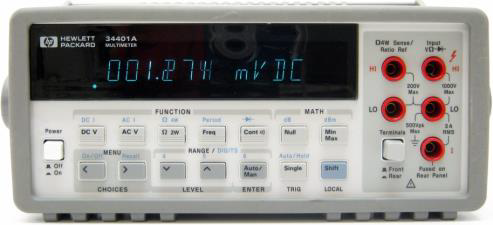
\includegraphics[width=0.5\linewidth]{fig/screenshot010}
	\caption{Multimetro Digitale}
	\label{fig:screenshot010.1}
\end{figure}
\end{adjustwidth}
\newpage
\subsubsection{Autoriscaldamento}	
\begin{adjustwidth}{2in}{}
		Come si tiene a bada l'autoriscaldamento? Questo infatti entra sempre in gioco come grandezza di influenza, è infatti causato da una corrente ed è inevitabile per misure in cui questa entra in gioco. 
		\begin{enumerate}
			\item Si aumenta lo scambio termico;
			\item Si diminuisce la tensione di alimentazione, ma questo implica una diminuzione della corrente sul circuito e quindi una diminuzione della sensibilità dello strumento. 
			\item  Si effettuano più misure variando la corrente e stimando la misura di resistenza a $ I=0 $.			
			\begin{figure}[H]
				\centering
				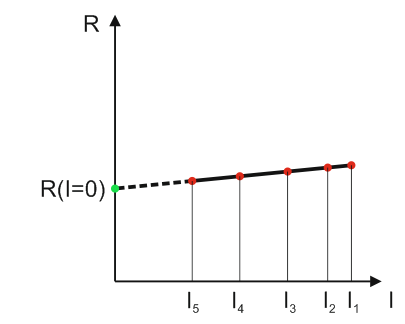
\includegraphics[width=0.5\linewidth]{fig/screenshot023(1)}
				\label{fig:screenshot0231}
			\end{figure}
			L'intercetta della retta di interpolazione di più misure, è la misura che sarebbe ottenuta senza lo scorrimento di corrente.
			
			\item Si usa una sorgente di alimentazione pulsata. Questa infatti permette il mantenimento di una elevata sensibilità limitando il calore dissipato.
\begin{figure}[H]
	\centering
	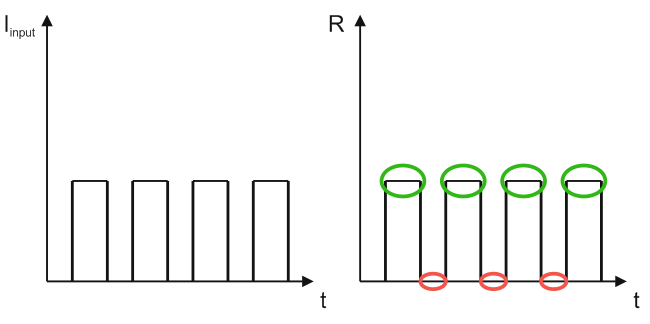
\includegraphics[width=0.5\linewidth]{fig/screenshot023(2)}
	\label{fig:screenshot0232}
\end{figure}
			Si usa in alimentazione un onda quadra e non si da il tempo alla corrente di scorrere in modo da non far instaurare l'effetto Joule. Si danno perciò una serie di ON-OFF in rapida successione in modo da non far surriscaldare le resistenze. 
			
			Il limite di questa misurazione è che è una misura discreta , non continua e costante. 
		\end{enumerate}
		 
\newpage

{\LARGE \textbf{NOTE}}
	
	%DA DECOMMENTARE PER AVERE LA VERSIONE STAMPABILE A DUE PAGINE 	
	%	\newpage
	%		\null
	%		\vfill
	%\begin{tcolorbox}[height=4.5cm]
	%	This box has a height of 4.5cm.
	%\end{tcolorbox}
	%		
\end{adjustwidth}
\end{document}